\section{Signal and backgrounds expectations}
\label{sec:MCexpectations}
% ---- ---- ---- ---- ---- ---- ---- ---- ---- ---- ---- ---- ---- ---- ---- ---- ---- ---- ---- ---- ---- ---- ----


\subsection {The signal}
% .... .... .... .... .... .... .... .... .... .... .... .... .... .... .... .... .... .... .... .... .... .... ....


Figure~\ref{fig:higgsXSBR} shows the trend of the Higgs cross section production and decay branching ratio into four fermions, 
as a function of its mass.
%
\begin{figure}[htb] 
  {\centering
    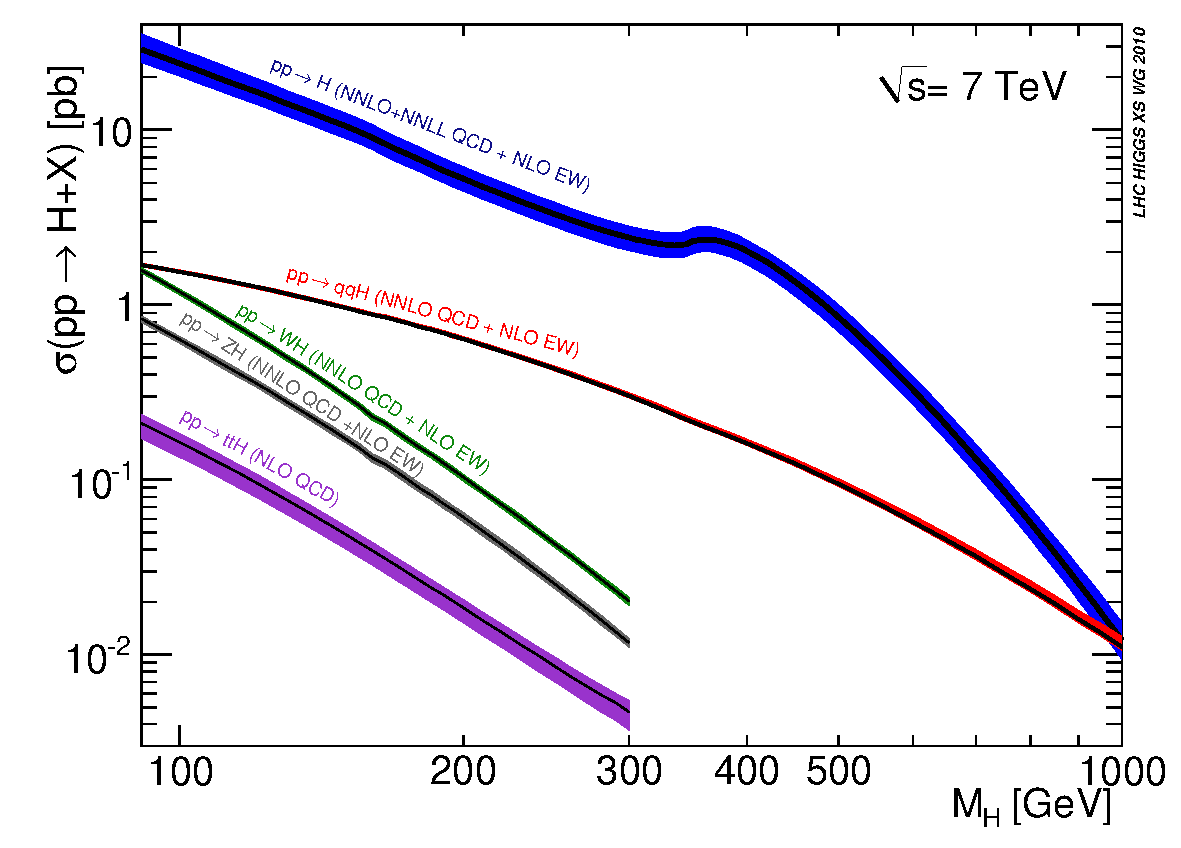
\includegraphics[width=0.54\textwidth]{plots/limitplot/Higgs_XS_7TeV.pdf}
    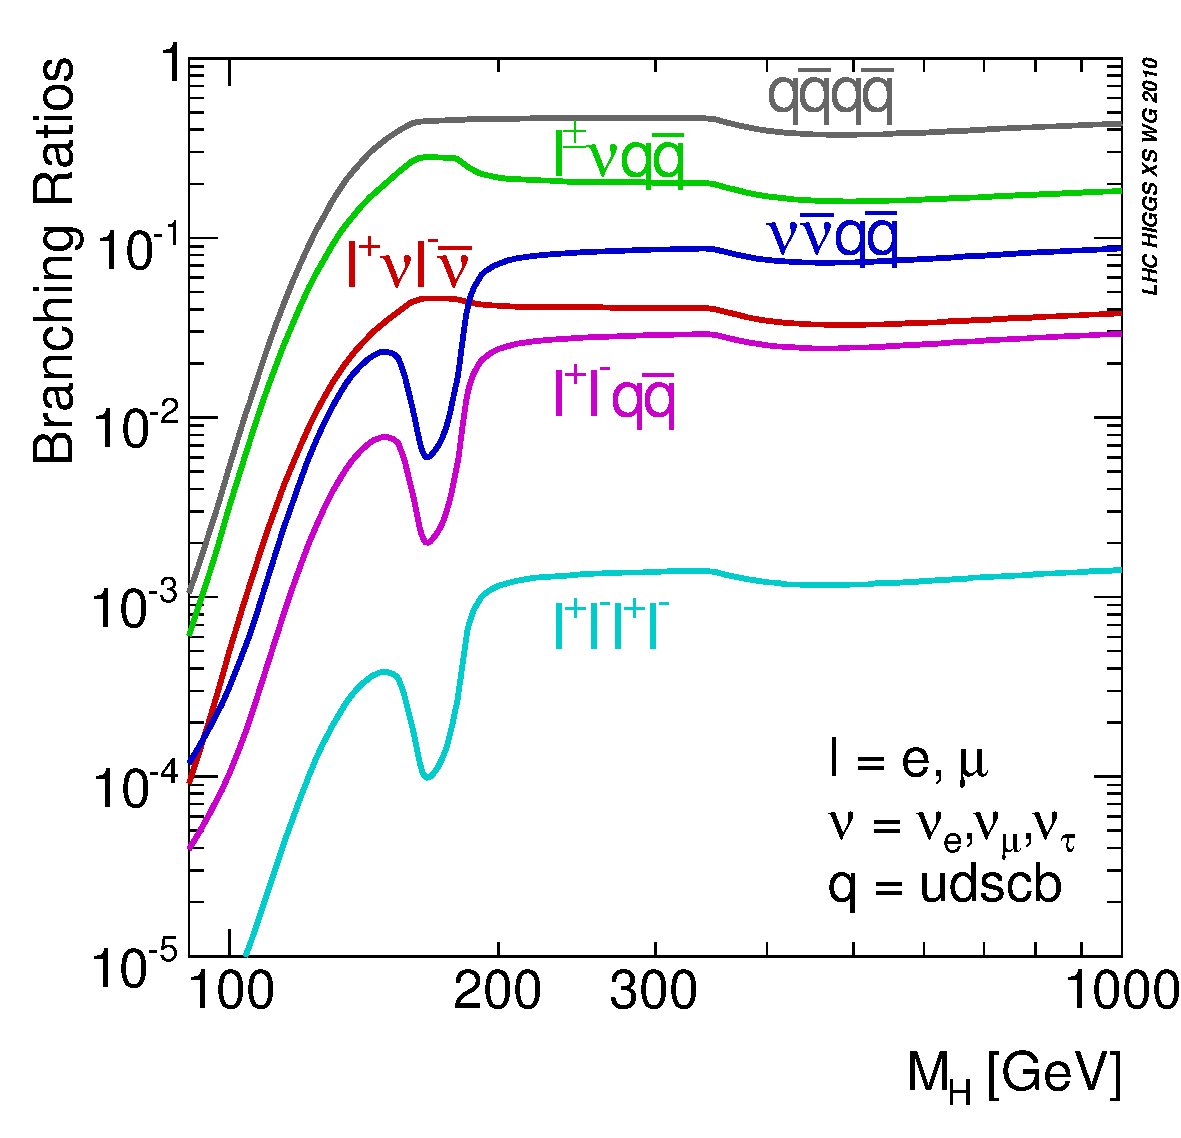
\includegraphics[width=0.42\textwidth]{plots/limitplot/Higgs_BR_4fermion_1.pdf}
    \caption{Standard Model Higgs boson production cross sections (left) and branching ratio into four fermion final states (right).}
    \label{fig:higgsXSBR}}
\end{figure}
%
The expected production cross-section, mutiplied by the branching fraction 
of the SM Higgs boson decay into a pair of W bosons \cite{LHCHiggsCrossSectionWorkingGroup:2011ti} 
and subsequently into a lepton-neutrino and di-jet pair, translates into the effective cross-section
for the analyzed process, as listed in Table~\ref{tab:signals} as a function of the Higgs mass.

\begin{table}[htb]
  \begin{center}
  \begin{tabular}{c|c|c}
  \hline
  $m_{\textnormal{H}}$ (\GeVcc) & $\sigma_{\textnormal{gg}}$ (pb) & $\sigma_{\textnormal{VBF}}$ (pb) \\
  \hline
%  160 & $2.41  \pm 0.45$          & $0.234^{+0.006}_{-0.006}$\\
  170 & $2.18  \pm 0.39$          & $0.230^{+0.008}_{-0.004}$\\
  180 & $1.85  \pm 0.33$          & $0.204^{+0.006}_{-0.004}$\\
  190 & $1.36  \pm 0.23$          & $0.159^{+0.005}_{-0.003}$\\
  200 & $1.12^{+0.19}_{-0.17}$    & $0.136^{+0.005}_{-0.003}$\\
  250 & $0.67^{+0.11}_{-0.10}$    & $0.087^{+0.003}_{-0.002}$\\
  300 & $0.48^{+0.08}_{-0.07}$    & $0.060^{+0.003}_{-0.002}$\\
  350 & $0.45^{+0.09}_{-0.07}$    & $0.0416^{+0.002}_{-0.0012}$\\
  400 & $0.34^{+0.05}_{-0.06}$    & $0.0272^{+0.0016}_{-0.0008}$\\
  450 & $0.22^{+0.03}_{-0.04}$    & $0.0197^{+0.0013}_{-0.0006}$\\
  500 & $0.13^{+0.02}_{-0.02}$    & $0.0150^{+0.0011}_{-0.0005}$\\
  550 & $0.084^{+0.016}_{-0.015}$ & $0.0117^{+0.0009}_{-0.0004}$\\
  600 & $0.053^{+0.010}_{-0.010}$ & $0.0093^{+0.0008}_{-0.0004}$\\
  \hline
  \end{tabular}
  \end{center}
  \caption{The cross section for the signal, where the branching fractions of the Higgs into WW
  and of each W into leptons are taken into account in the calculation.}
  \label{tab:signals}
\end{table}%


\subsection {The backgrounds}
% .... .... .... .... .... .... .... .... .... .... .... .... .... .... .... .... .... .... .... .... .... .... ....


All the processes with the presence in the detector of one lepton, two jets and missing energy
have to be considered as possible sources of background. The most relevant ones are:
% %FIXME in what order should we present it?
\begin{itemize}
  \item $W$+jets: this is the production of single $W$ vector bosons in association with quarks or gluons 
       that mimick the final state signature and the hadronic $W$ decay products.
       Because of its cross-section, 
       this is by far the most important backgruond to the analysis.
  \item Drell-Yan $Z/\gamma^{*}$+jets: this is the production of single $Z/\gamma^{*}$ bosons 
       in association with quarks or gluons, 
       where one lepton gets undetected because of acceptance or inefficiency effects, 
       and the hadronic activity mimicks the final state signature and the hadronic $W$ decay products.
       %FIXME One of the main handles to reduce this background is the low missing energy, the MZZ
  \item $WW$: this non resonant production is an irreducible background for the analysis.
  \item $WZ$: in case the $Z$ decays hadronically, or the $W$ decays hadronically 
              and one $Z$ lepton is not identified by the detector,
              this sample also contributes to the backgrounds.
  \item $ZZ$: in case one $Z$ decays hadronically, and one lepton is not identified by the detector,
              this sample contributes to the backgrounds.
  \item $t\bar{t}$: top quarks pairs are produced at LHC via the gluon fusion process
              $gg\to{}t\bar{t}$ or via QCD quark annihilation $qq\to{}t\bar{t}$.
              The semi-leptonic sample, where one $W$ decays hadronically,
              can be reduced by requests on the number of jets,
              while the fully leptonic one is reduced by requiring anly one good lepton in the event.
              In any case, 
              because of acceptance and inefficiencies, 
              this background still contaminates the signal phase space.      
  \item Single top production: it proceeds through three separate channels:
       \begin{enumerate}
         \item t-channel: top is produced after a quark-gluon interaction 
               with the exchange of a virtual $W$.
         \item s-channel: top is produced in association with an anti-bottom, 
               after the annihilation of a pair of quarks in a weak vertex.
         \item tW-channel: top is produced in association with a charged vector boson in a weak process, 
               from a gluon-bottom pair in the initial state.
       \end{enumerate}
%       The first two can be distinguished from signal thanks to a selection on the energy of b-quarks, 
%       which are quite different from signal tag quarks, while tW-channel has got a missing jet.
  \item QCD multi-jet events generate a background 
       because of the non-negligible probability of jets to be reconstructed as leptons.
\end{itemize}

The cross section for the backgrounds, multiplied by the branching ratio when meaningful, 
are reported in Table~\ref{tab:bkg_XS}. 
Each different sample notation includes all the decays taken into account 
in the effective cross section calculation.

\begin{table}[htb]
  \begin{center}
  \begin{tabular}{c|c}
  \hline
  Channel & Cross-section (pb) \\
  \hline
  W+jets                        & $31314  $ \\ %  \pm 1600 $ \\
  Z+jets                        & $3050   $ \\ %  \pm 130$ \\
  WW                            & $43     $ \\ %  \pm 1.5$ \\
  WZ                            & $18.2   $ \\ %  \pm 0.7$\\
  ZZ                            & $5.90   $ \\ %  \pm 0.15$\\
  t$\bar{\textnormal{t}}$+jets  & $157.5  $ \\ %  \pm 10$ \\
  t+jets ($t$-channel)          & $64.6   $ \\ % \pm 0.05$ \\
  t+jets ($s$-channel)          & $4.6    $ \\ % \pm 1.1$ \\
  t+jets ($t$W-channel)         & $15.7   $ \\ % \pm 0.8$ \\
  QCD (ele enriched)            & $6740000$ \\ % \pm $\\
  QCD (mu enriched)             & $84700  $ \\ % \pm $\\
  \hline
  \end{tabular}
  \end{center}
  \caption{The cross section for the backgrounds, multiplied by the branching ratio when meaningful.
  Each different sample notation includes all the decays taken into account in the calculation.}
  \label{tab:bkg_XS}
\end{table}%
